\documentclass[12pt]{amsart}
\usepackage{amsmath,amssymb,amsbsy,amsfonts,latexsym,amsopn,amstext,cite,
                                               amsxtra,euscript,amscd,bm}
\usepackage[colorlinks,linkcolor=blue,anchorcolor=blue,citecolor=blue,backref=page]{hyperref}
\usepackage{color}
\usepackage[T1]{fontenc}
\usepackage[utf8]{inputenc}
\usepackage{pgfplots}
\pgfplotsset{
	tick label style={font=\footnotesize },
	label style={font=\footnotesize},
}
\usepackage{tikz}

\begin{document}

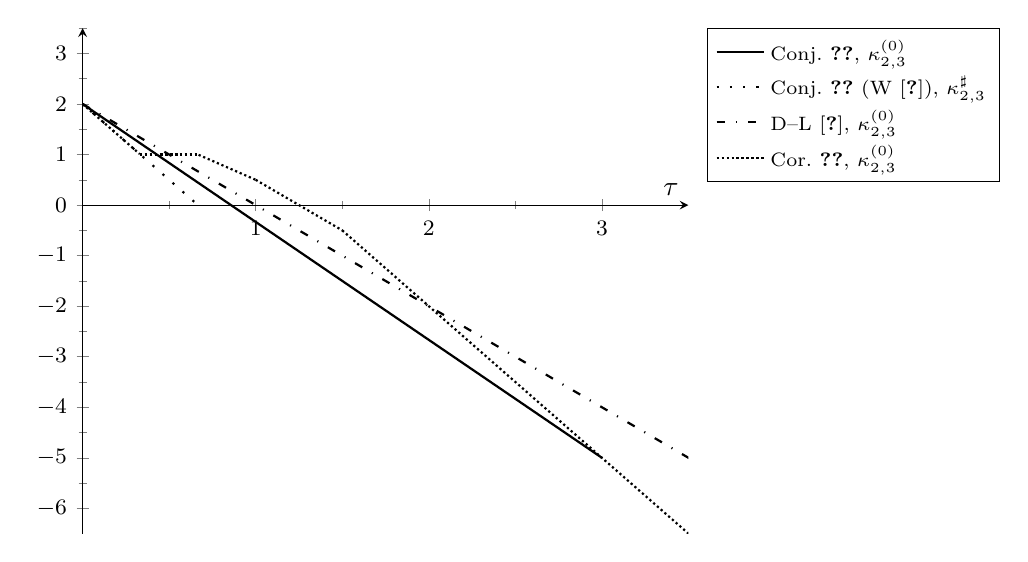
\begin{tikzpicture}
	\begin{axis}[
	xticklabels={$0$,$1$,$2$,$3$},
	yticklabels={${-6}$,$ {-5}$,$ {-4}$,$ {-3}$,$ {-2}$,$ {-1}$,$0$,$1$,$ 2$,$ 3$},
	axis x line=middle,
	axis y line=left,
	height=8cm,
	ytick pos=left,
	ytick={-6,-5,...,4},
	xtick={0,1,...,3},
	minor y tick num=1,
	minor x tick num=1,
	y label style={rotate=-90},
	xlabel={{$\tau$}},
	ymin=-6.5, ymax=3.5,
	xmin=0, xmax=3.5,
	legend style={
		cells={anchor=west},
		legend pos=outer north east,
	}
	]
	
	\addplot[solid,thick] expression[domain=0:3] {2-(7/3)*x};
	\addlegendentry{\scriptsize{Conj.~\ref{conj2},  $\kappa_{2,3}^{(0)}$}}
	
	\addplot[loosely dotted, thick] expression[domain=0:0.67] {2-3*x};
	\addlegendentry{\scriptsize{Conj.~\ref{conj:Wooley} (W~\cite{Wool3}), $\kappa_{2,3}^{\sharp}$}}	
	
	\addplot[loosely dashdotted, thick] expression[domain=0:4] {2-2*x};
	\addlegendentry{\scriptsize{D--L~\cite{DeLa},  $\kappa_{2,3}^{(0)}$}}	
	
	\addplot[densely dotted, thick]expression[domain=0:0.33] {2-3*x};
	\addplot[densely dotted,thick, forget plot]expression[domain=0.33:0.67] {1};   
	% need the "forget plot" so there's only one legend entry for both functions
	\addplot[densely dotted,thick, forget plot]expression[domain=0.67:1] {2-(3/2)*x};
	\addplot[densely dotted,thick, forget plot]expression[domain=1:1.5] {5/2-2*x};
	\addplot[densely dotted, thick, forget plot]expression[domain=1.5:4] {4-3*x};
	\addlegendentry{\scriptsize{Cor.~\ref{cor:mvt-weight-small d}, $ \kappa_{2,3}^{(0)}$}}
	
		
	\end{axis}
	\end{tikzpicture}

\end{document}